\documentclass[tikz,border=2pt]{standalone}
\usepackage{pgfplots}
\pgfplotsset{compat=1.18}
\usetikzlibrary{intersections}
\usepgfplotslibrary{fillbetween}


\begin{document}
	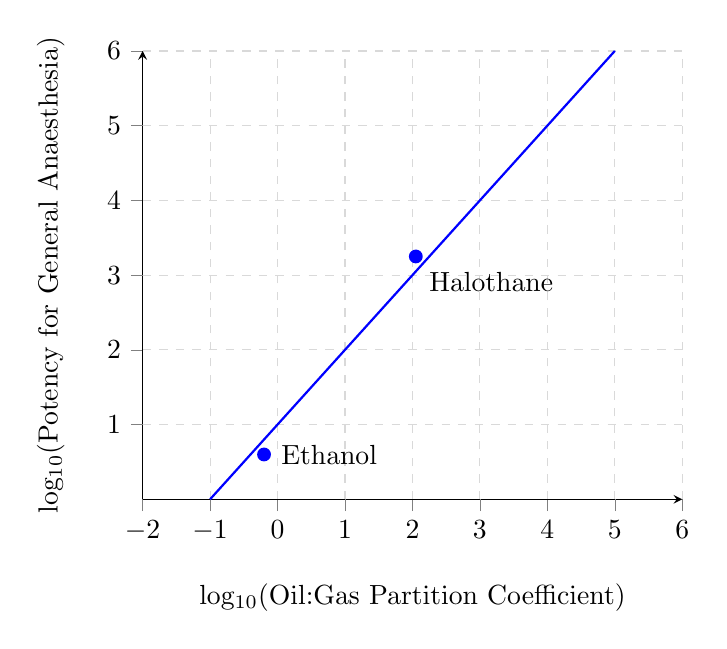
\begin{tikzpicture}
		\begin{axis}[
			axis lines=middle,
			ymin = 0,
			ymax = 6,
			xmin = -2,
			xmax= 6,
			grid = major,
			grid style={dashed, gray!30},
			ylabel near ticks,
			xlabel near ticks,
			extra y ticks ={1, 3, 5},
			extra x ticks = {-1,1,3,5},
			xlabel= log$_{10}$(Oil:Gas Partition Coefficient),
			ylabel= log$_{10}$(Potency for General Anaesthesia),
			tick align=outside,
        			axis y line shift=2,
			legend pos= south east,
			legend style={font=\small, cells={align=left}}]

			\draw [blue, thick] (-1,0) -- (5,6);

			\node[circle,fill=blue,inner sep=0pt, label={[text = black]300:Halothane}, minimum size = 5pt)] at (2.05,3.25) {};
			
			\node[circle,fill=blue,inner sep=0pt, label={[text = black]0:Ethanol}, minimum size = 5pt)] at (-0.2,0.6) {};


		\end{axis}
	\end{tikzpicture} 
\end{document}